\documentclass[journal]{IEEEtran}
\usepackage[pdftex]{graphicx}
\usepackage[cmex10]{amsmath}
\usepackage{ifthen}
\usepackage{stfloats}

% declare the path(s) where your graphic files are
\graphicspath{{./diagrams/}}

\begin{document}

% paper title
% can use linebreaks \\ within to get better formatting as desired
\title{Dynamic Load Balancing for\\Heterogeneous Systems}

% author names and IEEE memberships
\author{Kenneth~Lee,~Kyle~Morgan}%

% The paper headers
\markboth{CS 5504: Computer Architecture}{Final Project Paper, 5 December 2011}

% make the title area
\maketitle

\begin{abstract}
Leveraging maximum performance from specialized hardware is one of the
major problems facing computer scientists today.  General-purpose computing
on graphics processing units (GPGPU) is a technique that is becoming
increasingly popular for handling computations typically performed by the
CPU.  However, many GPGPU algorithms place the entire workload on the Graphics
processing unit (GPU) leaving the CPU idle for the duration of the computation.
This paper investigates the effect various load-balancing schemes across the CPU
and GPU have on overall application performance.  Additionally, the discrete and
fused GPU architectures, and their impact on performance, will be investigated.
\end{abstract}

\section{Introduction}
% The very first letter is a 2 line initial drop letter followed
% by the rest of the first word in caps.
% 
% form to use if the first word consists of a single letter:
% \IEEEPARstart{A}{demo} file is ....
% 
% form to use if you need the single drop letter followed by
% normal text (unknown if ever used by IEEE):
% \IEEEPARstart{A}{}demo file is ....
% 
% Some journals put the first two words in caps:
% \IEEEPARstart{T}{his demo} file is ....
\IEEEPARstart{L}{everaging} the maximum performance from specialized hardware is one
of the major problems facing computer scientists today.  The unique architecture of the
GPU gives it a place as a massively parallel hardware accelerator.  Programming frameworks
such as OpenCL allow programmers to utilize the stream processors of the GPU for non-graphics
data.  However, because of the difficulty in programming for this hardware, most of the
effort is spent on trying to achieve performance from the GPU, while the CPU is left
unused.  By also making use of CPU to process a chunk of the data, we can achieve higher
utilization of resources and therefore increase overall program performance.

GPU+CPU co-processing hardly a new idea.  Jimenez et al.~\cite{Jimenez2009} present a
dynamic library which can be used in a system to dynamically schedule tasks for GPU
computation across various processes. The method described only looks at optimizing
usage of the GPU across the whole system, rather than optimizing a single applications
performance. The StarPU system, on the other hand, presents a method of co-processing
and load balancing on a per application basis~\cite{Augonnet2009}. They show that by
using an appropriate model for the load balancing, they are able to achieve improvements
in speed for applications which call for code acceleration multiple times.  We intend
to extend this work to improve the speed of each kernel execution by splitting the
work of that kernel over the capable resources, similar to the schemes used by
OpenMP~\cite{Dagum1998}. Both of these papers address data transfer times as a major cost
of GPU computing. Using the new AMD Fusion architecture, which fuses the CPU and GPU onto
a single die, we may be able to eliminate or greatly reduce this cost, which will impact
the overhead of GPU+CPU co-processing.

We expect that by using GPU+CPU processing we will improve the performance of the
application, when compared to CPU-only or GPU-only.  That is, consider a workload of size
$n$, a GPU that requires $t_g$ time to perform one block of computation, and a CPU that
requires $t_c$ time to perform one block of computation. We expect that the GPU would
require time $nt_g$ to perform a given computation, while the CPU would require $nt_c$
time to perform the same computation.  Optimally, we would expect the load-balancing
scheme to require the following time to perform the computation.
\[\max{\{(n-m)t_g, mt_c}\} + t_d + t_o\]
Where $m$ is the amount of the workload given to the CPU ($m \leq n$), $t_d$ is the data
transfer cost, and $t_o$ is any overhead incurrent from synchronization costs of the load
balancing scheme or otherwise.  The above will be faster than just the GPU iff
$t_g - \max{\{(n-m)t_g, mt_c}\} < t_d + t_o$.

Two different load balancing schemes were implemented for this paper.  The first was a
static load balancer, which partitions the workload in two, and transfers one chunk to
the CPU, and the other to the GPU.  The CPU and GPU work entirely independently, and
their results are merged once each finish.  The static load balancer should have no
synchronization overhead, and transfers all of the data prior to the computation.
The main caveat with a static load balancer is that the ratio of the workload given to
the CPU is chosen by the load balancer.  An optimal ratio would be one such that the
time to perform the computation is equal for both the CPU and GPU.  Unfortunately, this
optimal ratio will be application-dependent, meaning that a fixed ratio cannot be optimal
for every application.  In order for a static load balancer to be optimal for a given
application, a programmer must tune the amount of workload given to the CPU that works
best for that application.

The second scheme is a dynamic load balancer, which partitions the data into many smaller
chunks.  One chunk is sent to the CPU and GPU each for computation.  When one finished,
it requests another chunk from the load balancer, and this process repeats until the
entirely workload has been sent to either the CPU or GPU.  The dynamic load balancer
will incur some amount of synchronization overhead, because shared variables that track
which chunks of the workload are left must be protected by a lock.  Unlike the static
load balancer, the dynamic load balancer transfers data throughout the computation.
The dynamic load balancer is designed to mitigate the primary problem with the static
load balancer -- that the optimal ratio of computation performed on the CPU is
application-dependent.  A chunk size must be chosen such that the processing units are
not requesting chunks so frequently that contention for shared variables rise and
synchronization overhead increases, yet small enough to not allow one processing unit
to receive a disproportionate amount of work.

\section{Architecture Overview}
In this section we discuss the different architectures of the experimental
machines under test.  We will discuss CPU, GPU, and APU architectures in
terms of major differences that affect the performance of the device.  

\subsection{CPU Architecture}
The CPU architecture is designed as a low latency architecture.  To facilitate
the needs for low latency application performance, a series of hierarchical 
caches have been designed to hide memory access costs, the most common cause
of latency in single-threaded applications on modern architectures.  Each core
of the CPU typically only runs one or two hardware-enabled threads to reduce
cache pollution, thus avoiding latency.  An simplistic example CPU architecture is given
by Figure~\ref{fig:cpu_arch}.

The use of the Single Instruction Multiple Data (SIMD) paradigm enables increased
performance on these devices by increasing data throughput for data parallel
applications.  However, optimal performance of these types of instructions often
involves complex compilation techniques and hand-tuning of the assembly.

\subsection{GPU Architecture}
The GPU almost acts a foil to the CPU architecture.  Instead of optimizing the
architecture of the device to increase performance of a single thread, the GPU
architecture is specifically designed for large throughput performance.  Large
numbers of threads can be easily created an run on a GPU.  Large register files
enable tens of thousands of threads to be run on today's GPU architecture with
very little penalty for context switching.

Groups of processing units, Streaming Multiprocessors (SMs), share a single instruction
dispatch unit and operate in lock step.  The threads themselves run on each SM
in a group, called a warp, typically of 32 threads.  Because of these architectural
features divergent branching in a warp (caused by if-else clauses) greatly degrade application
performance.

The memory architecture for the GPU is very different than that found on the CPU. 
Instead of a large hierarchy of caches to hide memory latency for single thread
performance the latency to memory is instead hidden through aggressive context
switching.  Newer GPU architectures may contain privative caching schemes.
Each SM on the GPU also contains a local memory memory space which can accessed 
at much lower latency .  This memory space is typically used as a user-managed
cache. The memory hierarchy for the GPU architecture is given by Figure~\ref{fig:gpu_arch}.

\begin{figure}[t]
\centering
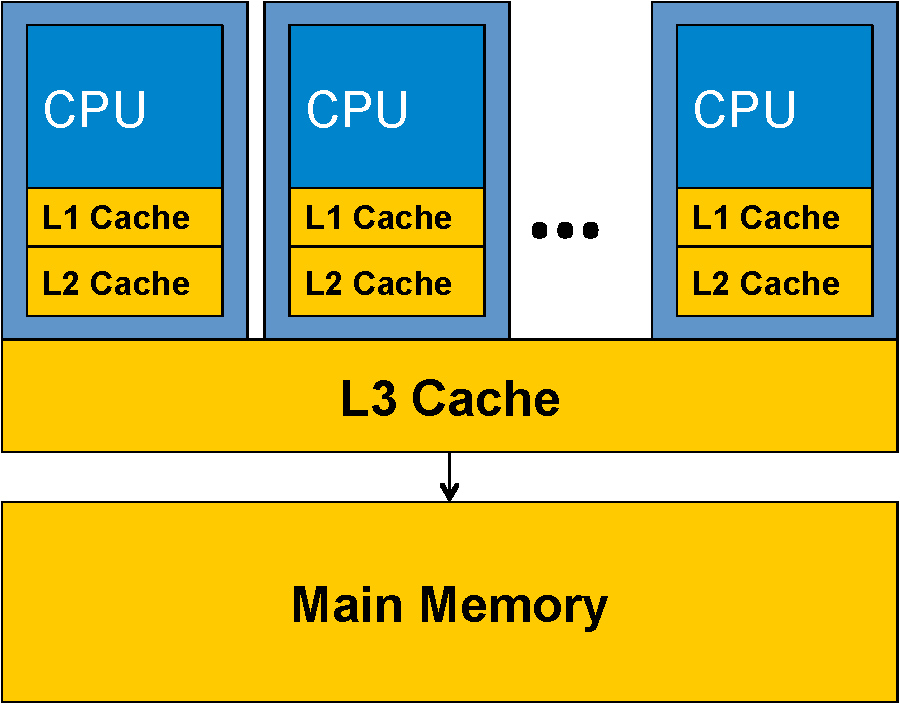
\includegraphics[width=2.5in]{cpu_architecture}
\caption{CPU Architecture}
\label{fig:cpu_arch}
\end{figure}

\begin{figure}[t]
\centering
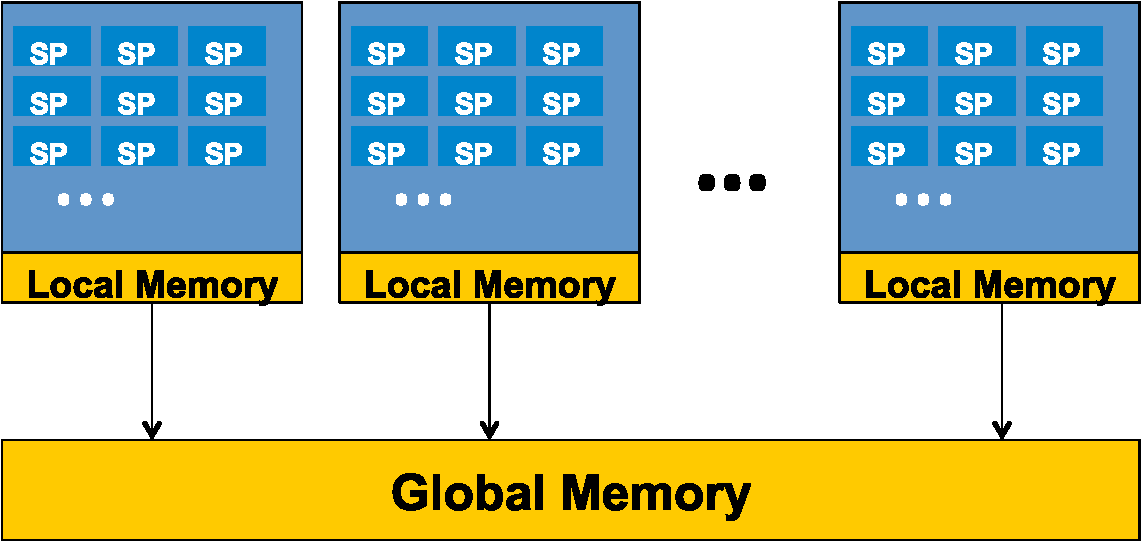
\includegraphics[width=2.5in]{gpu_architecture}
\caption{GPU Architecture}
\label{fig:gpu_arch}
\end{figure}

\subsection{APU Architecture}
The APU is a relatively new, novel architecture that attempts to 
improve on the the discrete CPU+GPU system.  The CPU die is split
between the typical CPU processor as well as allocating space
for a SIMD engine, the basis for a GPU processor.  The APU has a 
shared memory between the CPU and SIMD engine, in which accesses
are facilitated through a high-speed memory controller.  The AMD
Fusion technology is an example of this type of architecture~\cite{AMDFusion}.

One of the main benefits of the APU is the elimination of the PCI-e
bus, which allows for much faster transfer between CPU and GPU.  Daga et al.
show that the AMD Fusion architecture allows for much faster data transfers
between CPU and GPU, allowing for an overall improvement in runtime, despite
reduced compute power on the GPU~\cite{Daga2011}. 

\section{Load Balancing Benchmarks}
For this paper, three different benchmarks were used to assess the
effectiveness of the load balancer.  The first is a reduction benchmark,
in which the sum of variably-sized array is computed.  The reduction benchmark
is unique in that different code is being run on the CPU and the GPU.  The
reason for this is that the GPU cannot efficiently compute a reduction the way
a CPU typically would -- due to the relative inefficiency of backward branches
on the GPU.  A reduction on the GPU is a multi-stage process, in which the
output of one step is used as the input of the next.  Each steam processor
computes the reduction of two elements during each iteration, reducing the amount
of work during each step by a factor of two.  As a result, each step utilizes half
the stream processors of the previous step.  This continues until the reduction
operation is only done by a single stream processor.  A natural consequence of
this algorithm is that not all of the stream processors will be utilized during
the computation.

The next benchmark is a simple vector addition operation that computes the sum
of two input vectors, and stores the result into an output vector.  The third
benchmark, referred henceforth as the ``Vector Add+'' benchmark, is similar to
the Vector Add benchmark, but it computes 1000 additions before storing the result
in the output vector.  The motivation behind this benchmark is to reduce memory
access overhead with more computation.  All numbers reported in the results section
are given as a mean of ten runs for that particular benchmark, load-balancing scheme,
and data size.

\section{The OpenCL Framework}
For this project, we will use the OpenCL Framework for our kernel lauching.  OpenCL
is an application framework for heterogeneous parallel computing.  It includes an
API for creating and transferring memory to accleration devices, as well as dynamic
compilation of application kernels that are run on the acceleators.Using OpenCL 
allows us to write the host code only once, while allowing us to run the core 
application kernel on the CPU, GPU, or both.

In OpenCL each thread is logically mapped to a work-item.  These work-items are grouped into
workgroups.  These workgroups map to a SM on a discrete GPU.  For instance, these workgroups
share access to a SMs local memory and can perform a barrier with all the other work-items
in the workgroup.  In the case of a CPU acclerator, the workgroups still exist, but optimizations
such as manual caching via local memory will not be effective.

Devices are grouped into contexts, which contains memory buffers and so on.  A queuing system
is used by OpenCL to facilitate kernel execution.  Kernels are submitted to the queue along with
the size of each workgroup, as well as number of workgroups to execute.  This queue is also 
responsible for reading and writing memory buffers.  The queue is in-order, meaning that 
the queue will wait until previously enqueued items have finished before starting work 
on more recently queued items.

For our purposes, we decided to use a seperate context for each device, as well as a seperate
command queue for each context.  We decided to use a seperate context for each device, as it would
allow for finer-grained control of data transfers and residency. Using a seperate command queue
for each device will facilitate multiple devices to be used simultaneously, as each command queue
operates on its own seperate thread.

\section{Load Balancing Schemes}
A naive implementation of CPU+GPU co-processing will in many cases lead to an imbalance
of work for either the CPU or GPU.  To deal with this problem we will investigate the
use of 2 different load balancing schemes in addition to the performance of a CPU-only or
a GPU-only solution.  These schemes are illustrated in Figure~/ref{fig:scheduling}

The first load balancing scheme that was implemented was a static division of work between
the CPU and the GPU at a specified ratio.  This ratio was user-defined allowing for best 
performance after runtime benchmarking (i.e. the precentage of work done on the CPU and GPU).
The cases of CPU-only and GPU-only scheduling are just special cases of this scheduler, of
the ratios 0 and 1 respectively.

The static load-balancing scheme benefits from the low overhead of only have to launch the
kernels on each device only once, as opposed to more complex load-balancing schemes.  This
increases the amount of work to be done at one time, as workgroups that retire are immediately
replaced by newer workgroups from the larger queue. The main cause of overhead for this method
of load-balancing is that of a varying workload.  If the workload for the kernel is imbalanced
between workgroups, it is impossible to statically determine the proper amount of work
to put on each kernel.  Improper allocation of work to each device will not allow both
devices to be fully utilized, and application performance will not be optimal.

To address the issue of a dynamic work load between workgroups for kernels, we also used
a dynamic load-balancing scheme.  In this scheme the workgroups were grouped into larger
chunks.  Each device is initially allocated one chunk of work to work on, and as each chunk
is retired by the device a new chunk is allocated.  Each device is given a seperate hardware
thread, and the thread will wait until the current chunk is finished, then it will synchronize
through a shared variable to acquire the next chunk of work for the device.  This process
will continue until the work queue is out of work. 

The dynamic load-balancing scheme will still not guarantee optimal performance.
Within a work chunk, a single long-running workgroup can hold up the entire device,
not allowing other kernels to execute on open SMs.  This creates and issue where the
size of the work chunks should be considered.  One one hand, larger work chunks can
provide for better performance for each device, as it will allow more workgroups to
hide the cost of a long-running workgroup.  However, large chunk sizes can reduce
the granularity of load-balancing between the devices.

\begin{figure}[t]
\centering
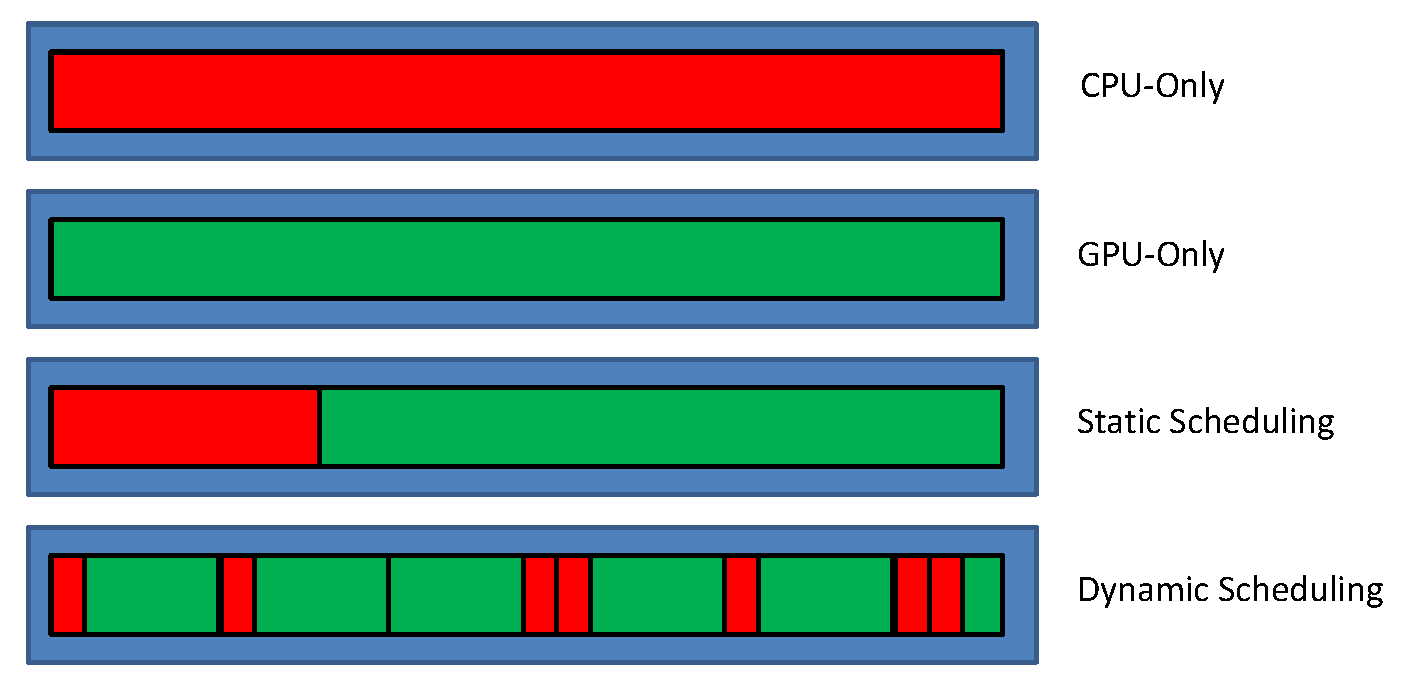
\includegraphics[width=2.5in]{scheduling}
\caption{Data Partitioning Schemes for Load Balancing.}
\label{fig:scheduling}
\end{figure}

\section{Results and Analysis}
We tested the different benchmark applications using different hardware environments.
For the discrete GPU tests, we tested our application on an Intel Core Duo CPU with a
AMD HD5450 GPU attached via PCIe.  For the Fused CPU+GPU environment we used an AMD
Fusion A-3850.  Linux was used for the discrete environment, while Windows was used
on the Fused environment (in order to take advantage of newer drivers that allowed
for better hardware features on the new Fusion machine).  

The three implemented benchmarks were run on a system with a discrete GPU, as well as
on a fused GPU platform.  In dynamic load balancing benchmarks, a chunk size of 80~KB
was used.  Dynamic results are only given for the discrete GPU testing environment,
as the APU platform was running Windows and our code was written with POSIX compliance
in mind.  In static load balancing benchmarks, the ratio of data computed on the GPU
will be specified.

\begin{figure}[t]
\centering
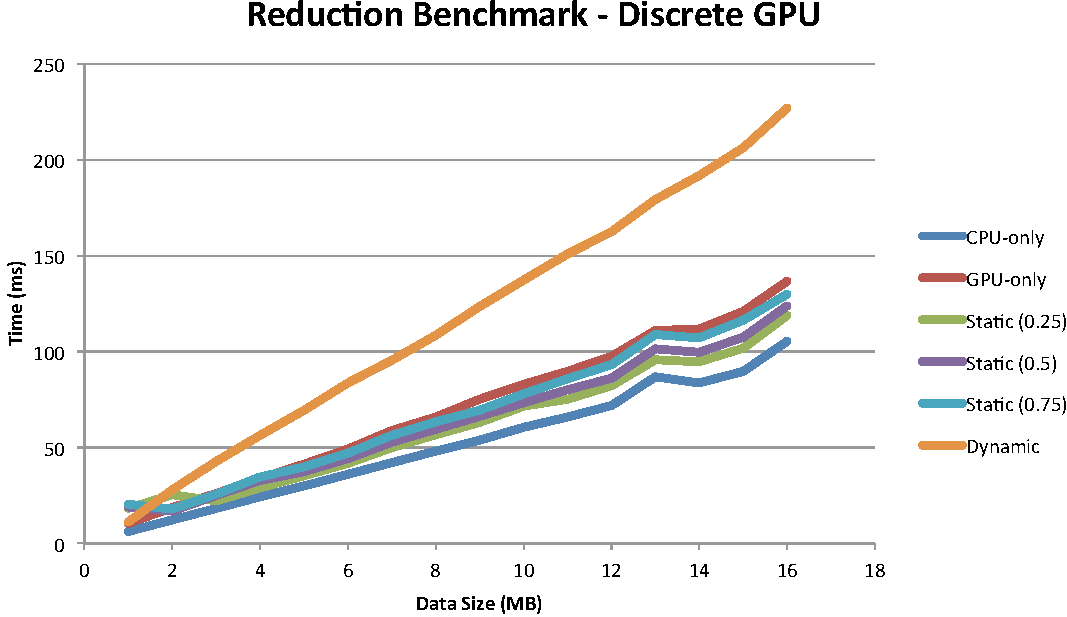
\includegraphics[width=3.0in]{reduce_discrete}
\caption{Reduction Benchmark on a Discrete GPU Platform}
\label{fig:reduce_discrete}
\end{figure}

First, the reduction benchmark was run on the discrete GPU platform with a variety of
different data sizes and load balancing policies, as shown in Figure \ref{fig:reduce_discrete}.
Interestingly, the CPU outperformed the GPU on this particular benchmark.  This is likely
due to the GPU not utilizing all of its stream processors during a reduction operation, as
discussed previously.  Unfortunately, none of the static load balancing schemes were able
to outperform just the CPU; all the static times were somewhere in between the CPU-only and
GPU-only times.  Additionally, the dynamic load balancing scheme performed significantly
worse than all the other schemes, and more than 100\% worse than just the CPU.
100\% worse than just the CPU.

\begin{figure}[t]
\centering
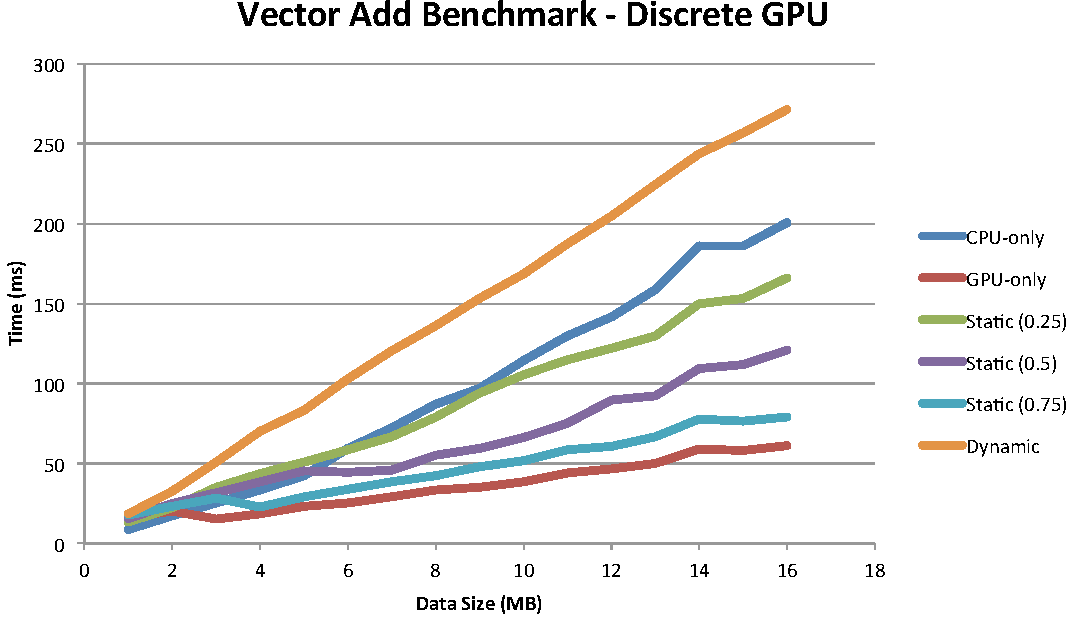
\includegraphics[width=3.0in]{vector_discrete}
\caption{Vector Add Benchmark on a Discrete GPU Platform}
\label{fig:vector_discrete}
\end{figure}

Now, consider Figure \ref{fig:vector_discrete}, where the vector add benchmark was run on
the discrete GPU platform.  In this case, we see that the GPU has nearly a 4x speedup over
just the CPU.  However, similar to the reduction benchmark, the static load balancing schemes
never outperform just the GPU alone, with all of them lying somewhere between the CPU-only
and GPU-only runs.  Also similar to the reduction benchmark, the dynamic load balancing scheme
performs significantly worse than all the other schemes.

\begin{figure}[t]
\centering
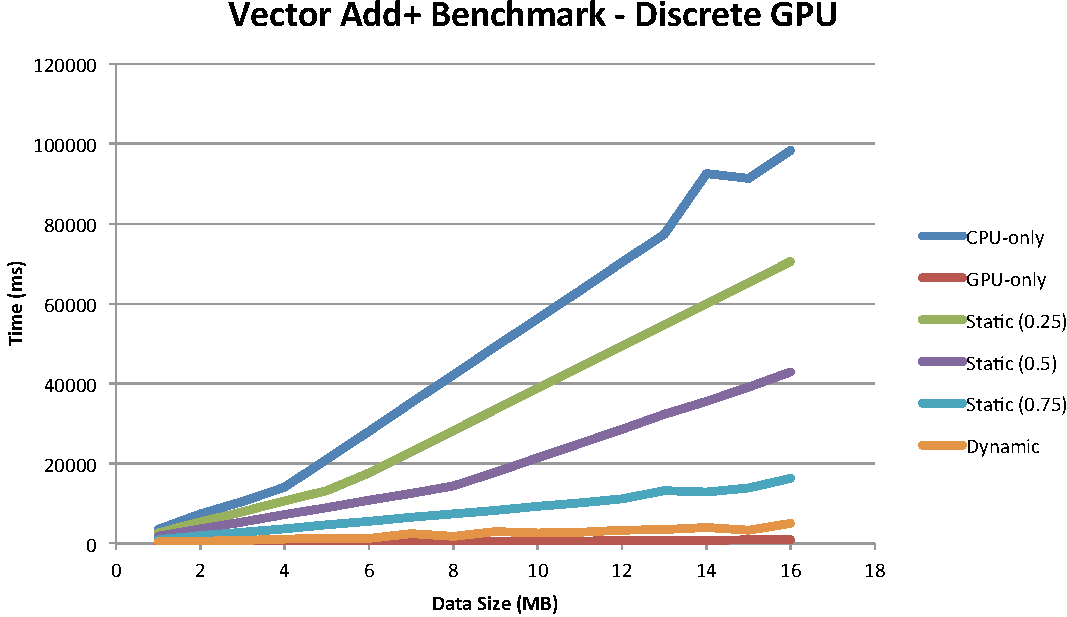
\includegraphics[width=3.0in]{vector_plus_discrete}
\caption{Vector Add+ Benchmark on a Discrete GPU Platform}
\label{fig:vector_plus_discrete}
\end{figure}

The results for the vector add+ benchmark on the discrete GPU platform are shown in Figure
\ref{fig:vector_plus_discrete}.  There are a few notable trends in this figure that are not
present in the previous two.  The first is is how drastically the GPU outperforms the CPU --
with over a 100x speedup over just the CPU with 16~MB of data.  The second is that the
dynamic load balancing drastically outperforms the static load balancing schemes.  This is
almost certainly because the GPU so drastically outperforms the CPU.  With the dynamic load
balancing scheme, only small chunks of data are given to the CPU at a time, rather than a
static percentage.

\begin{figure}[t]
\centering
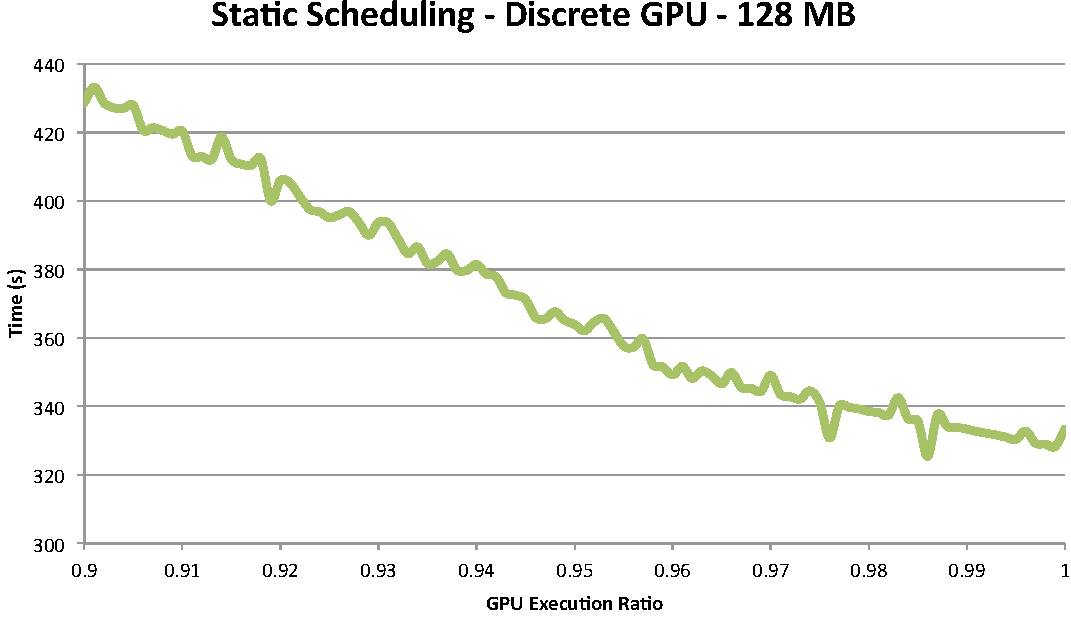
\includegraphics[width=3.0in]{static_discrete}
\caption{Varying Data Ratio with a Discrete GPU}
\label{fig:static_discrete}
\end{figure}

For the above figures, the static load balancer was run with three different
data ratios run on the GPU -- 25\%, 50\%, and 75\%.  The general trend was that
as more of the workload was placed on the GPU, the runtime improved.  As a
result, we run the vector add benchmark again with a high granularity of data
ratios.  Figure \ref{fig:static_discrete} shows  this benchmark on the discrete
GPU platform with between 90\% and 100\% of the data on the GPU, with a 0.1\%
granularity.  The total execution time, including data transfers, has an
obvious downward trend as more of the data is executed on the GPU.  That said,
there are a couple of static ratios which yielded better performance than
executing all of the data on the GPU.  Most notably, when only 98.6\% of the
data was executed on the GPU.  In this instance, the overall execution time was
325.27 seconds, compared to 333.31 seconds with only the GPU -- a ~2.4\%
speedup.  However, these few instances of speedup may simply be due to variability.

\begin{figure}[t]
\centering
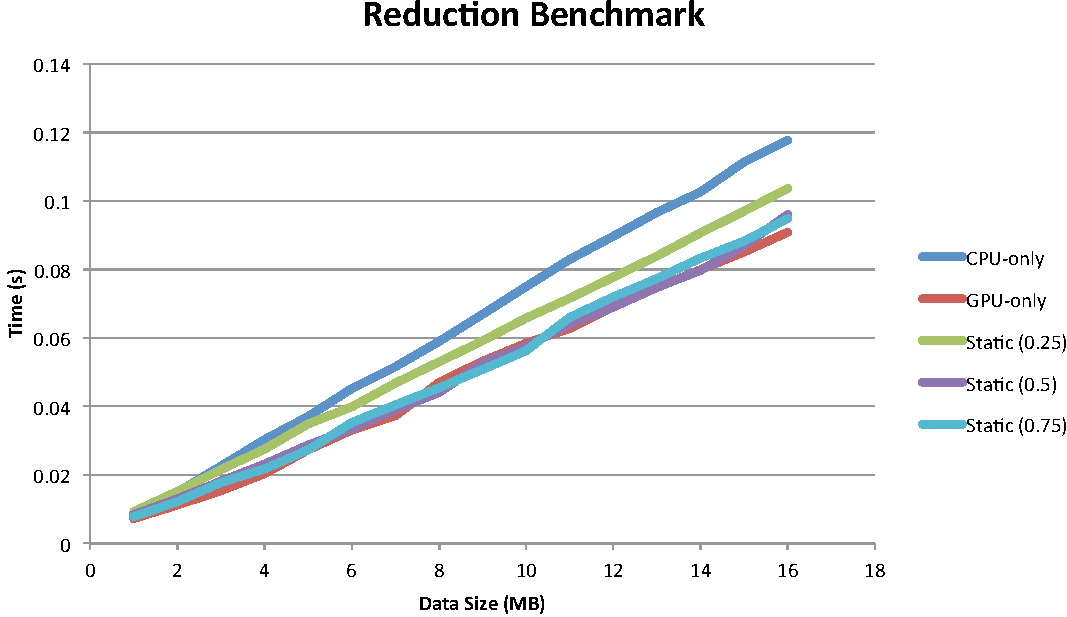
\includegraphics[width=3.0in]{reduce_fused}
\caption{Reduction Benchmark on a Fused CPU+GPU Platform}
\label{fig:reduce_fused}
\end{figure}

\begin{figure}[t]
\centering
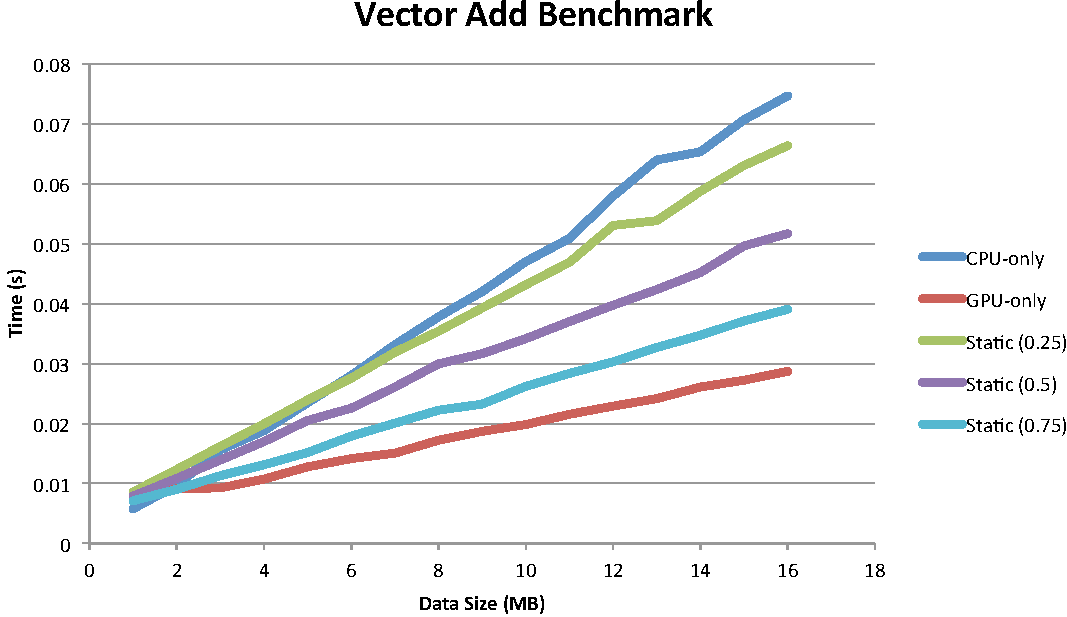
\includegraphics[width=3.0in]{vector_fused}
\caption{Vector Add Benchmark on a Fused CPU+GPU Platform}
\label{fig:vector_fused}
\end{figure}

\begin{figure}[t]
\centering
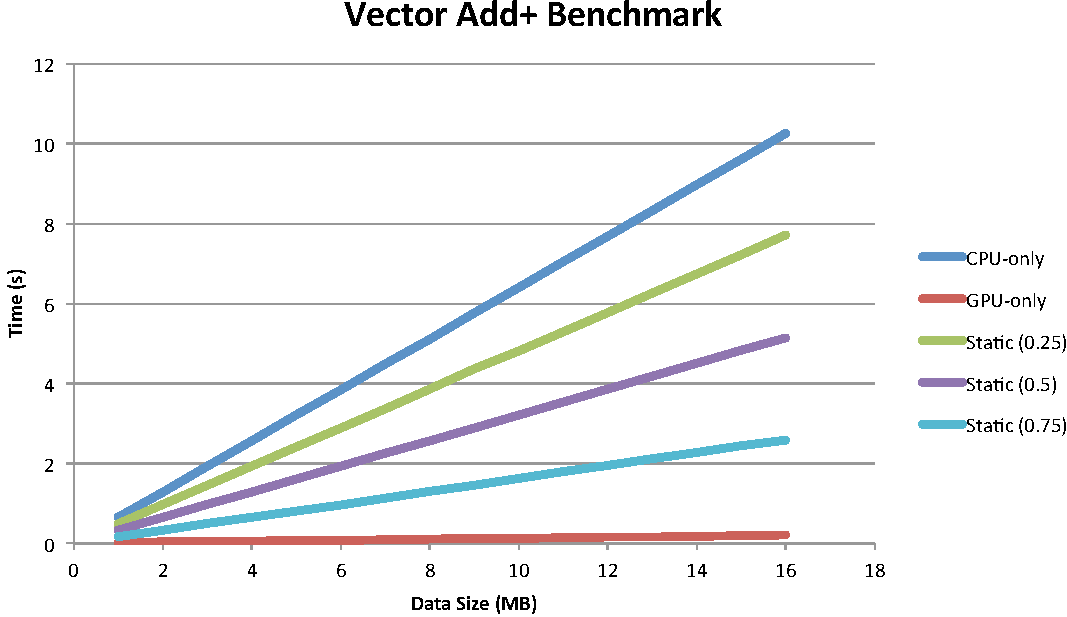
\includegraphics[width=3.0in]{vector_plus_fused}
\caption{Vector Add+ Benchmark on a Fused CPU+GPU Platform}
\label{fig:vector_plus_fused}
\end{figure}

Next, consider Figures \ref{fig:reduce_fused}, \ref{fig:vector_fused}, and
\ref{fig:vector_plus_fused}. The figures demonstrate a variety of different
load balancing options for the Reduction, Vector Add, and Vector Add+
benchmarks, across data sizes ranging between 1~MB and 16~MB.  Each figure
depicts the total execution time for the CPU-only and GPU-only computations,
as well as static load balancing with 25\%, 50\%, and 75\% of the data on the
GPU.  In each of the figures, it's evident that the GPU performs significantly
faster than the CPU for the given benchmarks, with the static partitioning
schemes lying somewhere between the two.

The only deviation from the above is the reduction benchmark, in which the GPU
only performs ~14\% faster than the CPU in the 16~MB case (0.104 seconds for the
GPU, 0.091 seconds for the CPU), and some of the static load balancing schemes
perform slightly better than just the GPU.  For instance, in the 9~MB and 10~MB
cases, both the 50\% and 75\% static schemes performed better than just the GPU
(0.5\% and 4.4\% respective speedups for 9~MB, 1.5\% and 3.6\% respective speedups
for 10~MB). What is also interested to note is that on the fused CPU+GPU architecture,
the GPU outperformed the CPU on the reduction benchmark.  However, the opposite was
true of the reduction benchmark on the discrete GPU platform.

%\begin{figure}[t]
%\centering
%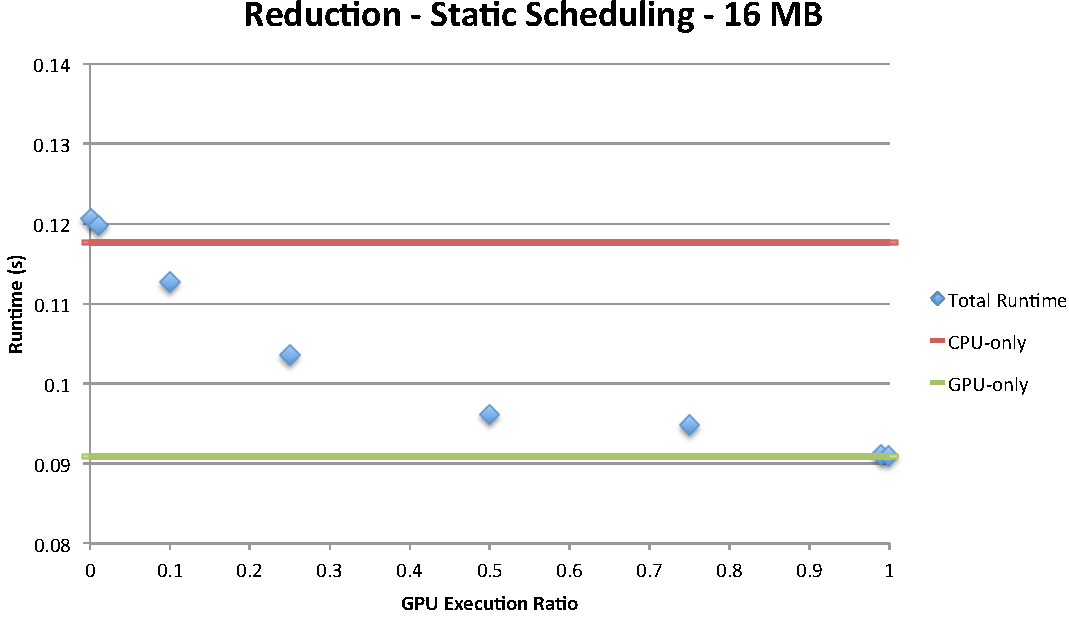
\includegraphics[width=3.0in]{reduce_static_fused}
%\caption{Reduction Benchmark with Varied Execution Ratio}
%\label{fig:reduce_static_fused}
%\end{figure}

%\begin{figure}[t]
%\centering
%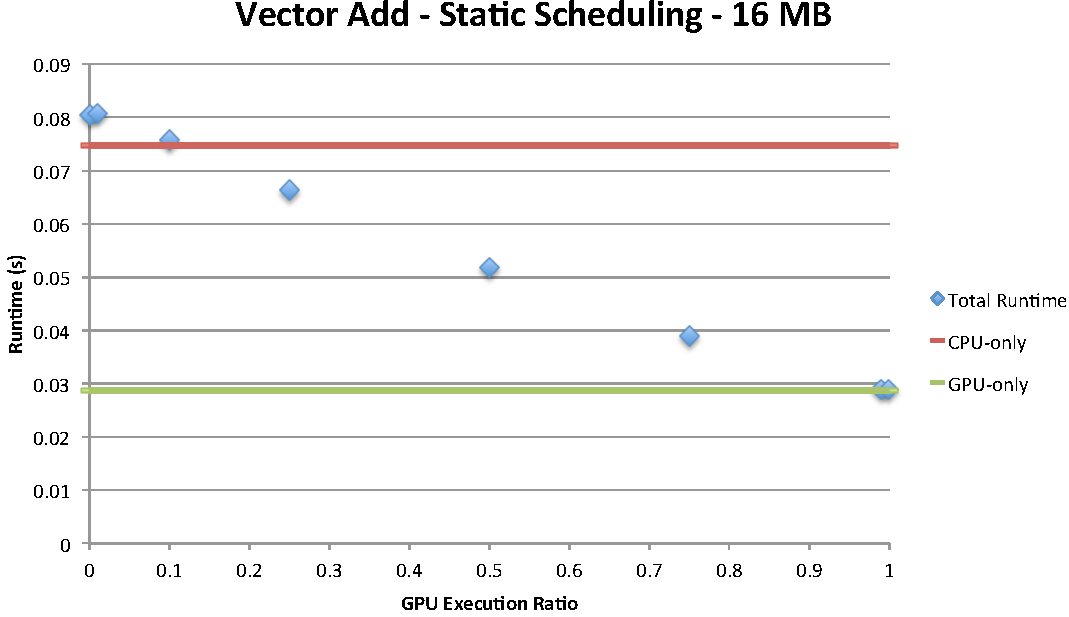
\includegraphics[width=3.0in]{vector_static_fused}
%\caption{Vector Add Benchmark with Varied Execution Ratio}
%\label{fig:vector_static_fused}
%\end{figure}

%\begin{figure}[t]
%\centering
%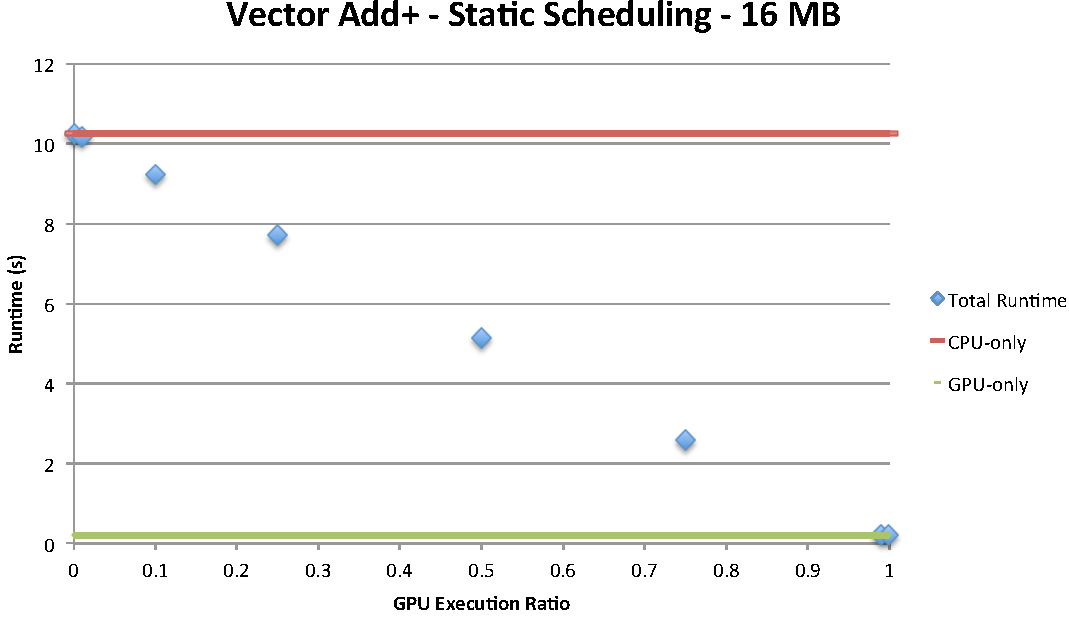
\includegraphics[width=3.0in]{vector_plus_static_fused}
%\caption{Vector Add+ Benchmark with Varied Execution Ratio}
%\label{fig:vector_plus_static_fused}
%\end{figure}

%Finally, consider Figures \ref{fig:reduce_static_fused}, \ref{fig:vector_static_fused},
%and \ref{fig:vector_plus_static_fused}. In each, the runtim for both the CPU and GPU are
%shown with a 16~MB problem size.  Additionally, a variety of static execution ratios are
%shown between 0.1\% and 99.9\%.  In every benchmark, none of the execution ratios were
%able to achieve a better time than just the GPU.

Based on the times shown in the previous figures, it is clear that the
static load balancing is ineffective at improving the overall efficiency
of any of the benchmarks tested.  There were a few scenarios in which
a specific static execution ratio achieved meager speedup ($<$5\%) over
just the GPU, but these situations were scarce, and did not achieve the
speedup we desired.  Additionally, this small amount of speedup would
require a significant amount of tine-tuning by a programmer.

Consider the 16~MB vector add benchmark, where the CPU-only case took
0.07465 seconds to run, and the GPU-only case took 0.02873 second to run.
Ideally, 72.2\% of the workload would be placed on the GPU, and 27.8\%
on the CPU.  Assuming no other overhead, this would result in an overall
runtime of 0.02075 seconds -- a 27.8\% speedup over the GPU.  Using similar
reasoning, a 43.6\% theoretical speedup is attainable for the reduction
benchmark.  A measly 2\% would be expected from the vector add+ benchmark,
because of the vast disparity in the CPU-only and GPU-only runtimes.

\begin{figure}[t]
\centering
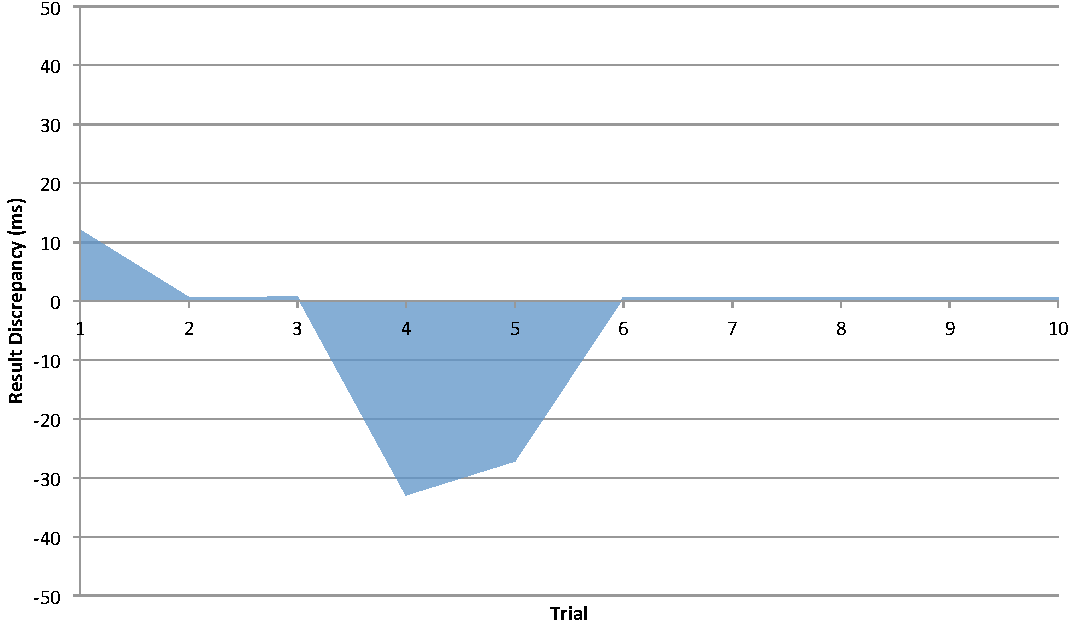
\includegraphics[width=3.0in]{sequential_discrepancy}
\caption{Discrepancies between expected runtimes and actual runtimes.}
\label{fig:sequential_discrepancy}
\end{figure}

The above results have lead us to believe that the CPU and GPU kernels are
not running truly in parallel as we initially believed.  As such, we used
an AMD profiler to report how long each of the kernels took using the static
load balancer with 95\% of the data on the CPU.  Figure \ref{fig:sequential_discrepancy}
shows the discrepancy between the actual total runtime of the vector add
benchmark and the expected runtime (that is, the sum of the CPU kernel runtime
and the GPU kernel runtime).  If the kernels were truly running in parallel,
we would expect to see a negative discrepancy between the actual runtime and
expected runtime.

Many of the trials produced a small positive discrepancy.  There were only
two trials which produced a negative discrepancy; however, these trials
were unusual in other ways as well.  The overall runtime of the CPU kernel
was rough 5.1~ms in all of the trials except these two, which were 36.6~ms
and 31.6~ms, respectively.  We believe that OpenCL is beginning the CPU
kernel, scheduling the GPU kernel before the CPU kernel has completed,
running the GPU kernel to completion, then scheduling the CPU kernel again
and letting it run to completion.  Thus, the profiler's record of the runtime
of the CPU kernel would include the runtime of the GPU kernel.

\section{Related Work}
Ryoo et al. discuss optimization strategies for GPU versus CPU runtime
systems~\cite{Ryoo2007}.  However, their research is based on a GPU-only
or CPU-only implementation instead of a heterogeneous approach.  The work
presented in ~\cite{Jablin2011} describes a runtime and compiled framework
for improving memory access latency and reducing data transfer overhead
for GPU kernels.  Our work differs from this, because the kernel execution
was still being performed solely on the GPU, whereas our work investigates
kernel execution on multiple devices.

Computation via heterogeneous systems is a relatively new research area for
high performance computing.  The various frameworks and large number of
different accelerator devices can make this quite difficult for application
programmers to manage.  The StarPU system~\cite{Augonnet2009} presents a 
framework to allow for programmers to write numerical codelets and have them
automatically run on a heterogeneous system.  Scheduling work for this system
is one of the most difficult parts of the system, because of the various
overheads for work-sharing schemes. We simplify this work, by looking at a
two-device system, and focus on the performance characteristics of different
scheduling scheme.  Verner et al. use this approach to create a high-throughput
low-latency heterogeneous encryption system~\cite{Verner2011}. 

Jimenez et al.~\cite{Jimenez2009} present a dynamic library which can be used
in a system to dynamically schedule tasks for GPU computation across various
processes. The method describes only looks at optimizing usage of the GPU across
the whole system, instead of optimizing a single application's performance.

% An example of a floating figure using the graphicx package.
% Note that \label must occur AFTER (or within) \caption.
% For figures, \caption should occur after the \includegraphics.
% Note that IEEEtran v1.7 and later has special internal code that
% is designed to preserve the operation of \label within \caption
% even when the captionsoff option is in effect. However, because
% of issues like this, it may be the safest practice to put all your
% \label just after \caption rather than within \caption{}.
%
% Reminder: the "draftcls" or "draftclsnofoot", not "draft", class
% option should be used if it is desired that the figures are to be
% displayed while in draft mode.
%
%\begin{figure}[!t]
%\centering
%\includegraphics[width=2.5in]{myfigure}
% where an .eps filename suffix will be assumed under latex, 
% and a .pdf suffix will be assumed for pdflatex; or what has been declared
% via \DeclareGraphicsExtensions.
%\caption{Simulation Results}
%\label{fig_sim}
%\end{figure}

% Note that IEEE typically puts floats only at the top, even when this
% results in a large percentage of a column being occupied by floats.


% An example of a double column floating figure using two subfigures.
% (The subfig.sty package must be loaded for this to work.)
% The subfigure \label commands are set within each subfloat command, the
% \label for the overall figure must come after \caption.
% \hfil must be used as a separator to get equal spacing.
% The subfigure.sty package works much the same way, except \subfigure is
% used instead of \subfloat.
%
%\begin{figure*}[!t]
%\centerline{\subfloat[Case I]\includegraphics[width=2.5in]{subfigcase1}%
%\label{fig_first_case}}
%\hfil
%\subfloat[Case II]{\includegraphics[width=2.5in]{subfigcase2}%
%\label{fig_second_case}}}
%\caption{Simulation results}
%\label{fig_sim}
%\end{figure*}
%
% Note that often IEEE papers with subfigures do not employ subfigure
% captions (using the optional argument to \subfloat), but instead will
% reference/describe all of them (a), (b), etc., within the main caption.


% An example of a floating table. Note that, for IEEE style tables, the 
% \caption command should come BEFORE the table. Table text will default to
% \footnotesize as IEEE normally uses this smaller font for tables.
% The \label must come after \caption as always.
%
%\begin{table}[!t]
%% increase table row spacing, adjust to taste
%\renewcommand{\arraystretch}{1.3}
% if using array.sty, it might be a good idea to tweak the value of
% \extrarowheight as needed to properly center the text within the cells
%\caption{An Example of a Table}
%\label{table_example}
%\centering
%% Some packages, such as MDW tools, offer better commands for making tables
%% than the plain LaTeX2e tabular which is used here.
%\begin{tabular}{|c||c|}
%\hline
%One & Two\\
%\hline
%Three & Four\\
%\hline
%\end{tabular}
%\end{table}


% Note that IEEE does not put floats in the very first column - or typically
% anywhere on the first page for that matter. Also, in-text middle ("here")
% positioning is not used. Most IEEE journals use top floats exclusively.
% Note that, LaTeX2e, unlike IEEE journals, places footnotes above bottom
% floats. This can be corrected via the \fnbelowfloat command of the
% stfloats package.



\section{Conclusion}
It is clear that our original hypotheses were not supported by our results.  That
is, we were not able to see consistent, significant speedup from any of our load
balancing schemes.  In many scenarios, the GPU simply outperformed the CPU, with
the static load balancing schemes falling somewhere between the two, and the dynamic
load balancer being far worse than anything else.  There were only two notable
exceptions to this trend.  The first was the reduction benchmark on the discrete GPU
platform, where the CPU outperformed the GPU due to the low stream processor utilization
inherent in a GPU reduction implementation.  However, the static load balancing schemes
were still outperformed by the CPU in this case, so no overall speedup was gained. The
second exception was the vector add+ benchmark on the discrete GPU platform, where the
dynamic load balancer actually outperformed the tested static load balancing schemes.
However, this was due to the vast disparity in the GPU and CPU runtimes for this
particular benchmark; giving any significant amount of data to the CPU would hurt
performance.  With the dynamic load balancer, the CPU will only compute a few blocks
of data, rather than 25\% or more with the static load balancer.

When analyzing more finely-grained static execution ratios, we found that, in the case
where the GPU outperforms the CPU, there is always a downward trend in overall runtime
as more data is executed on the GPU.  There were a couple sparse instances where a static
execution ratio performed better than using just the GPU, but we chalked these up to
typical variability in runtimes due to their infrequency and minute performance improvements.

When analyzing the results, we considered the possibility that the CPU and GPU kernels were
actually running in serial, which would explain the performance trends we were seeing in our
static and dynamic load balancing schemes.  An AMD profiler was used to find out the times each
kernel took to compute, and the sum of these times was compared to the actual runtime of the
benchmark.  We found that the actual runtime of the benchmark was typically slightly more than
the sum of the runtimes of each kernel, which seemed to indicate that the kernels were indeed
running serially, with some overhead for data transfer times.

Based on the CPU-only and GPU-only runtimes of each benchmark, we were able to calculate an
optimal static data partitioning, such that the computations on the CPU and GPU took equal
time to complete.  Based on the disparity of runtimes between the CPU-only and GPU-only
results, the optimal runtimes ranged from a 2\% to nearly a 45\% speedup over just the GPU
alone.  Unfortunately,


\begin{thebibliography}{1}

\bibitem{AMDFusion}
http://fusion.amd.com

\bibitem{Augonnet2009}
C.~Augonnet, S.~Thibault, R.~Namyst, and P.A.~Wacrenier,
``StarPU: A Unified Platform for Task Scheduling on Heterogeneous Multicore Architectures'' in
\emph{Proceedings of the 15th International Euro-Par Conference on Parallel Processing}, 2009, pp. 863-874.

\bibitem{Che2009}
S.~Che, M.~Boyer, J.~Meng, D.~Tarjan, J.W.~Sheaffer, S.H.~Lee, and K.~Skadron,
``Rodinia: A benchmark suite for heterogeneous computing'' in
\emph{Proceedings of the 2009 IEEE International Symposium on Workload Characterization (IISWC)}, 2009, pp. 44-54.

\bibitem{Daga2011}
M.~Daga, A.M.~Aji, and W.~Feng,
``On the Efficacy of a Fused CPU+GPU Processor (or APU) for Parallel Computing'' in
\emph{Application Accelerators in High-Performance Computing (SAAHPC)}, 2011, pp. 141-149.

\bibitem{Dagum1998}
L.~Dagum and R.~Menon,
``OpenMP: An industry-standard API for shared-memory programming'' in
\emph{IEEE Computational Science and Engineering} 1998, pp. 46–55.

\bibitem{Danalis2010}
A.~Danalis, G.~Marin, C.~McCurdy, J.S.~Meredith, P.C.~Roth, K.~Spafford, V.~Tipparaju, and J.S.~Vetter,
``The Scalable Heterogeneous Computing (SHOC) benchmark suite'' in
\emph{Proceedings of the 3rd Workshop on General-Purpose Computation on Graphics Processing Units}, 2010, pp. 63-74.

\bibitem{Jablin2011}
J.A.~Jablin, P.~McCormick, and M.~Herlihy,
``Scout: High-Performance Heterogeneous Computing Made Simple'' in
\emph{Parallel and Distributed Processing Workshops and Phd Forum (IPDPSW)}, 2011, pp. 2093-2096.

\bibitem{Jimenez2009}
V.J.~Jiménez, L.~Villanova, I.~Gelado, M.~Gil, G.~Fursin, and N.~Navarro,
``Predictive Runtime Code Scheduling for Heterogeneous Architectures'' in
\emph{Proceedings of the 4th International Conference on High Performance Embedded Architectures and Compilers}, 2009, pp. 19-33.

\bibitem{Ryoo2007}
S.~Ryoo, C.I.~Rodrigues, S.S.~Baghsorkhi, S.S.~Stone, D.B.~Kirk, and W.W.~Hwu,
``Optimization Principles and Application Performance Evaluation of a Multithreaded GPU Using CUDA'' in
\emph{Proceedings of the 13th ACM SIGPLAN Symposium on Principles and practice of parallel programming}, 2007, pp. 73-82.

\bibitem{Verner2011}
U.~Verner, A.~Schuster, and M.~Silberstein,
``Processing data streams with hard real-time constraints on heterogeneous systems'' in
\emph{Proceedings of the international conference on Supercomputing}, 2011, pp. 120-130.

\end{thebibliography}

\newpage
\appendix[Team Member Contributions]
Kenneth Lee did A, B, C.  Kyle Morgan did X, Y, Z.
\end{document}
